\documentclass[a4paper, 12pt]{report}
%\setcounter{chapter}{1}
\renewcommand\thesection{\arabic{section}}
\renewcommand{\contentsname}{Cuprins}
\renewcommand{\figurename}{Figura}
\renewcommand{\tablename}{Tabel}

\setcounter{tocdepth}{6}
\setcounter{secnumdepth}{6}

\usepackage{url}
\usepackage{hyperref}
\usepackage[backend=bibtex, style=numeric, citestyle=numeric, backref=true ,sorting=none]{biblatex}
\addbibresource{bibliography.bib}

\usepackage{indentfirst}
\usepackage[nobottomtitles*]{titlesec}

\usepackage{graphicx}
\usepackage[center]{caption}
\usepackage{caption}
\usepackage{subcaption}
\usepackage[export]{adjustbox}
\graphicspath{ {./images/} }


\usepackage[margin=3.2cm]{geometry}
%\usepackage[none]{hyphenat}

\usepackage{mathtools}

\usepackage{listings}
\usepackage{color}
\usepackage{float}

\definecolor{codegreen}{rgb}{0,0.6,0}
\definecolor{codegray}{rgb}{0.5,0.5,0.5}
\definecolor{codepurple}{rgb}{0.58,0,0.82}
\definecolor{backcolour}{rgb}{0.96,0.96,0.96}

\lstdefinestyle{mystyle}{
	backgroundcolor=\color{backcolour},   
	commentstyle=\color{codegreen},
	keywordstyle=\color{blue},
	numberstyle=\tiny\color{codegray},
	stringstyle=\color{codepurple},
	basicstyle=\fontsize{10}{10}\selectfont\ttfamily,
	breakatwhitespace=false,         
	breaklines=true,                 
	captionpos=b,                    
	keepspaces=true,                 
	numbers=left,                    
	numbersep=2pt,                  
	showspaces=false,                
	showstringspaces=false,
	showtabs=false,                  
	tabsize=2
}

\lstset{style=mystyle}

\usepackage{pythonhighlight}

\usepackage{fontspec} % -> LuaLatex
\setmainfont{UT Sans}

\usepackage{setspace}
\setstretch{1.1}


\begin{document}
	
	\begin{titlepage}
	
	\vspace*{-3cm}
	\hspace{-2cm}
	
\includegraphics[width=0.8\linewidth]{./images/Logo-UT-MI-SPOT-RO}

	\begin{center}
		\Huge
		
		\vspace{2cm}
		
		\textbf{Lucrare Dizertație}
		
		\vfill
				
		\Large
		\begin{tabular}{ll}
			\textbf{Autor:}&Hanganu Bogdan\\
			\textbf{Coordonator:}&Lect. Univ. Băicoianu Alexandra
		\end{tabular}
		
		\vfill
		
		\Large
		Brașov\\
		Iulie 2022
        
	\end{center}
\end{titlepage}
	\begin{titlepage}
	
	\vspace*{-3cm}
	\hspace{-2cm}
	
\includegraphics[width=0.8\linewidth]{./images/Logo-UT-MI-SPOT-RO}
	
	\begin{center}
		\Huge
		
		\vspace{2cm}
		
		\textbf{Lucrare Disertație}
		
		\vspace{1cm} 
		
		\LARGE Detectarea emoțiilor din perspective multiple
		
		\vfill
		
		\Large
		\begin{tabular}{ll}
			\textbf{Autor:}&Hanganu Bogdan\\
			\textbf{Coordonator:}&Lect. Univ. Băicoianu Alexandra
		\end{tabular}
		
		\vfill
		
		\Large
		Brașov\\
		Iulie 2022
		
	\end{center}
\end{titlepage}
	\newpage
	\tableofcontents
	\newpage
	\pagenumbering{arabic}
	\section{Abstract}	
	Această lucrare de disertație este elaborată în jurul problematicii identificării emoțiilor unei persoane. Utilizând metode de învățare automată, datele sunt înregistrate prin intermediul unor canale multiple (audio, video și text). 
	
	Expresiile faciale, obținute prin intermediul canalului video, reflectă în mod intuitiv starea mentală a unei persoane, fiind una dintre cele mai bogate și importante forme de comunicare inter-umană. Tonalitatea vocii care se adresează în timpul comunicării ne poate oferi informații valoroase referitoare la starea de spirit. Mesajul care este transmis prin intermediul vocii, ne oferă informații referitoare la personalitatea individului, fiind de ajutor mai departe în procesul de analiză.
	Datele stocate sunt mai apoi prelucrate folosind tehnici de procesare specifice fiecărui canal. Pentru input-ul audio este folosită procesarea digitală de semnal, cu următoarele tehnici reprezentative: Transformata Fourier, Transformata Fourier pe termen scurt, Coeficienți Mels. Procesare de imagini pentru canalul video vine în adăugare cu: scalare de date, transformare imaginii în greyscale, iar pentru text este de menționat: tokenizare, lematizare. Fiecare bloc de date preprocesat în mod corespunzător canalului părinte, va trece mai departe prin pasul de recunoaștere cu ajutorul metodelor de învățare automată.
	
	
	În această lucrare au fost realizate o serie de experimente pentru: procesarea datelor, antrenarea modelelor de machine learning. Finalizarea acestor teste a avut ca urmare dezvoltarea aplicației "Multimodal Emotion Detection" care să vină în sprijinul procesului de intervievare.
	\clearpage
	
	\section{Introducere}
	Aplicația "Multimodal Emotion Detection" are ca audiență persoanele care doresc să facă o analiză a candidatului care a trecut printr-un proces de intervievare. Fiind scrisă în limbajul de programare Python, permite o manevrare concisă a datelor inregistrate, care pot fi mai apoi vizualizate de către utilizator prin intermediul framework-ului GUI (Graphical User Interface) Qt.
	
	În cadrul lucrării, se propune recunoașterea emoțiilor utilizatorului într-un mod inteligent, utilizând tehnici și metode de machine learning si deep learning. Aceste două procedee sunt subcategorii ale domeniului numit inteligență artificială (IA), domeniu care a început să se modeleze si dezvolte în funcție de nevoile oamenilor.
	
	Dezvoltarea rapidă a inteligenței artificale, "Big data science" și a tehnologiei "Block chain" a provocat multiple schimbări în structura socială umană. În majoritatea proceselor unde este nevoie de interacțiune umană, se implementează automatizări care să sporească eficiența, să folosească resursele umane, software și hardware în mod cât mai eficace. La nivel industrial, sistemele automatizate inteligente sunt deja folosite in uzine, frabici, având rolul de a asigura în permanență buna funcționare a întregului ansamblu. Atât eficiența cât și performanțele acestor sisteme sunt motivate de către costul redus de mentenanță. La un nivel mai aproape de către utilizatori, putem realiza că inteligența artificială a început tot mai des să facă parte din viața de zi cu zi, ajungând în stadiul să devină indispensabil oamenilor.
	
	În zilele noastre, interacțiunea dintre oameni și IA este în continuă creștere, ajungand să intre treptat în viața noastră de zi cu zi. De la asistenți virtuali (care au rolul de a sprijini utilizatorul prin intermediul interpretării comenziilor vocale), până la reclame personalizate, aceste sisteme inteligente interacționează din ce în ce mai mult cu ființe umane. Deoarece este un subiect în care interesul este unul foarte crescut, relația între om și mașinăria inteligentă poate să ajungă la un nivel mai inalt, prin integrarea cu emoțiile utilizatorului. Acesta este un domeniu crucial de cercetare, oferind diverse oportunități și aplicări pentru oameni.
	
	Astfel, în următorul capitol va fi explicat despre fiecare din cele trei tipuri de recunoaștere a emoției utilizate, precum și modul în care acestea interacționează cu utilizatorul. Vor fi prezentate exemple de alte categorii a recunoașterii de emoții, care nu au fost încadrate în această lucrare, precum și aplicațiile care sunt deja în domeniul comercial și sunt utilizate.
	
	\clearpage
	\section{Recunoașterea emoțiilor}
	În general, o relație între doi indivizi se bazează pe încredere și întelegere. Pentru a putea crea un parteneriat, un algoritm inteligent trebuie să fie cabail să înțeleagă emoțiile umane. Emoția este un factor important atât în comunicarea verbală, cât și în comunicarea nonverbală (gesticulare, expresiile corpului). Identificarea stărilor unei persoane poate ajuta o mașină să înțeleagă intențiile utilizatorului, în scopul de a-i oferi o interacțiune mai potrivită. Printe primele studii care au fost făcute pentru integrarea sistemelor inteligente cu emoțiile umane, aceastea s-au reflectat în identificarea emoțillor prin voce, deoarece comunicarea verbala este una dintre cele mai rapide forme de socialiare, cu cel mai mare impact in istorie.
	
	Fiind una dintre cele mai consacrate aptiduni prin care o ființă inteligentă s-a putut diferenția și avansa în lanțul trofic, comunicarea verbală reprezintă un semnal complex, în care sunt transmise informații referitoare la mesaj, legate de emițător precum și de emoțiile transmise de acesta. Fiind o serie complexa, capacitatea sistemului care face identificarea emotiilor trebuie sa fie pe măsură, pentru a analiza cu acuratețe starea subiectului, oferindu-i astfel o experiență cât se poate de autentică. Nu numai atât, utilizând o astfel de recunoaștere, poate ajuta la crearea unor interfețe usor navigabile ("Recunoașterea emoțiilor prin vorbire este deosebit de utilă pentru aplicațiile din domeniul interacțiunii om-mașină deoarece ajută la crearea unor interfețe usor de utilizat"\cite{emotion_recognition_survery}).
	
	Deoarece semnalul audio conține și alte informații precum emoția transmisă de către emițător, algortimul de recunoaștere a emoțiilor umane prin extragerea trăsăturilor acustice capturate în vorbire, devine "baza pentru realizarea unei interacțiuni om-calculator mai armonioasă și mai eficientă, având o mare importanță în cercetare, precum și aplicativă"\cite{audio_emotion_recognition0}.
	
	În cadrul aplicației, vocea utilizatorului (semnalul audio) este folosită în doua contexte. Primul este dat de către identificarea emoțiilor candidatului pe baza a diferite trăsături acustice depistate din voce iar al doilea de către identificarea cuvintelor rostite, pentru a putea fi transformate în text. Deoarece în aplicatie identificarea textului (speech-to-text) este utilizat prin intermediul unor apeluri de tip API Rest la functionalitățile oferite de către Google, accentul se va pune pe prima utilizare în lucrare. Emoțiile care pot fi identificate în cadrul acestei recunoașteri sunt următoarele: furie, dezgustare, frică, fericire, tristețe, surprindere, neutral.
	
	Seviciului oferit de către Google pentru recunoașterea textului \cite{google_speech_to_text} este folosit cu scopul de a facilita identificarea personalității și a emoției transmise în urma interviului de către utilizator. Recunoașterea emoțiilor din text este în mod fundamental o problemă de clasificare pe baza conținutului, care include noțiuniuni de procesare de text (NLP, acronim de la "natural language processing"), precum și din domeniul deep learning. Modelul utilizat pentru acest tip de predicție este "The Big Five personality traits"\cite{big_five_personality_wiki}. 
	
	\begin{figure}[h]
		\begin{center}
			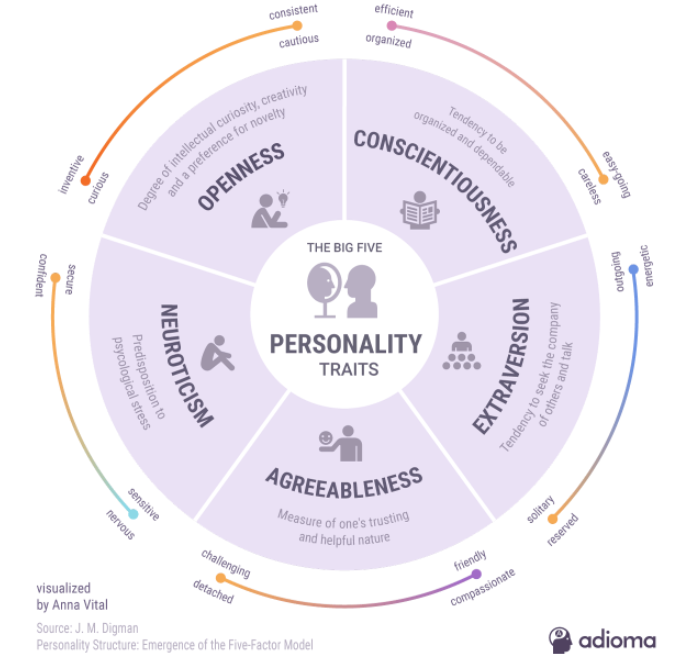
\includegraphics[scale=0.7]{images/ocean.png}
		\end{center}
		\caption{Cele cinci mari trăsături de personalitate\newline
			\hspace{\linewidth}https://blog.adioma.com/5-personality-traits-infographic/}
		\label{fig:ocean}
	\end{figure}
	
	În zilele noastre, se consideră că există 5 categorii de personalități (Figura \ref{fig:ocean}), având acronimul OCEAN. Mai jos, vom prezenta aceste personalități de bază:
	\begin{itemize}
		\item Deschidere (Openness): această trăsătură prezintă caracteristici precum imaginația și perspicacitatea. Oamenii care au punctat mai mult în această trăsătură tind să aibe o arie mai mare de interese. Sunt curioși de fire, dornici să dobândească aptitudini noi și să se bucure de orice experiență acumulată.
		
		\item Conştiinciozitate (Conscientiousness): printre caracteristicile de baza ale acestei trăsături, putem include un nivel ridicat de atenție, control bun al impulsurilor și comportamente care coduduc spre îndeplinirea obiectivelor. Oamenii care se încadrează acestei categorii tind să fie mai organizați și atenți la detalii. Ei planifică din timp, se gândesc la modul în care comportamentul lor îi afectează pe alții și sunt atenți la termenele limită.
		
		\item Extraversie (Extraversion): se caracterizează prin excitabilitate, sociabilitate și cantități mari de expresivitate emoțională. Oamenii care au un nivel ridicat de extraversie tind să capete energie în situații sociale. A fi în preajma altor persoane îi ajută să se simtă plini de energie și entuziasm.
		Oamenii care au un nivel scăzut de extraversie (sau introvertiți) tind să fie mai rezervați și au mai puțină energie în mediile sociale. În urma evenimentelor sociale se pot simți extenuați, iar introvertiții necesită adesea o perioadă de singurătate și tăcere pentru a își putea "reîncărca bateriile".
		
		\item Agreabilitate (Agreeableness ): pentru această personalitate, sunt incluse atribute precum încrederea, altruismul, bunătatea, afecțiunea și alte comportamente pro-sociale. Oamenii cu grad ridicat de agreabilitate tind să fie mai cooperativi, în timp ce aceia care au punctat mai slab pentru acest atribut, tind să fie competitivi și uneori chiar manipulativi.
		
		\item Nevrotism (Neuroticism): este un atribut caracterizat prin tristețe, melancolie și inconsevcență emoțională. Persoanele care au această trăsătură au tendința de a experimenta schimbări de dispoziție, anxietate, iritabilitate și tristețe. Aceia care au punctat scăzut în acest caz, tind să fie mai stabili și rezistenți emoționali.
	\end{itemize} 
	
	Nu în cele din urmă, dupa procesul de recunoaștere a trăsăturilor și emoțiilor transmise din voce, mai apoi interpretate în mod contextual prin procesare de text, urmează recunoașterea emoțiilor din cadrul expresiilor faciale. Pentru a putea fi în stare să facem o astfel de analiză, este nevoie identificarea unui chip uman (în engleză "face detection"). Pentru a facilita acest proces, prin intermediual camerei web care ne oferă flux de date video, biblioteca OpenCv\cite{open_cv} ne oferă suport pentru mijloace de identificare a fețelor candidaților. Având acest rezultat intermediar, este posibilă recunoașterea emoțiilor pe baza expresiilor faciale. Principalele stări emotive din cadrul fluxului video sunt aceleasi ca cele din audio.
	
	Făcând un ansamblu al componentelor descrise mai sus, acestea se unifică în ceea ce vom numi "Modulul de intervievare". În cadrul acestui modul, predicțiile pentru componentele audio și video sunt făcute live, iar in cazul textului, este realizat la final pentru a avea o cantitate mai ridicată de date, obținânand astfel o predicție cât mai aproape de adevăr.
	
	Tipurile de identificare a emoțiilor utilizate și descrise mai sus sunt doar câteva modele existente prin care o aplicație/mașină inteligentă poate interacționa în mod personalizat cu utilizatorul. Printre alte tipuri care merită menționate se enumeră gesturile corpului (limbajul corpului), fiind un subiect mai puțin explorat. Chiar dacă este un aspect important al psihologiei umane, primule studii moderne au devenit populare debia în 1960. Probabil cea mai importantă lucrare publicată înainte de secolul al XX-lea a fost "Expresia emoțiilor la om și la animale", scrisă de Charles Darwin \cite{human_body_lang_darwin}.
	
	În acest domeniu, după o cercetare a pieței care construiesc software-uri în jurul predicției emoțiilor, putem considera aplicațiile menționate mai jos ca fiind similare cu cea prezentată în această lucrare:
	\begin{itemize}
		\item Noldus Solutions Emotion Analysis cu "FaceReader™" \cite{noldus}: este un software specilizat pe analizarea datelor de tip imagine (atât din video cât și statice). Este un sistem robust, capabil să recunoască un număr de proprietăți specifice în imaginile faciale, inclusiv cele șase expresii de bază sau universale: fericit, trist, furios, surprins, speriat și dezgustat.
		\item iMotions cu "Facial Expression Analysis" \cite{imotions}: este un software specializat atât în analiza imaginilor cât și a datelor biosenzoristice. Modulul oferă 20 de măsuri de expresie facială (unități de acțiune), 7 emoții de bază, repere faciale, indici comportamentali, cum ar fi orientarea capului și atenția.
	\end{itemize}
	
	Diferența pe care o aduce aplicația prezentată în lucrare curentă, "Multimodal Emotion Detection",  este reprezentată de capacitate recunoașterii în timp real a emoțiilor prin intermediul altor input-uri, precum și a feedback-ului constant. Un alt aspect important prin care se diferențiază aplicația în cauză este dat de "Modulul de vizualizare a raportului", prin care se poate vedea la fiecare segment de date, textul care a fost spus, emoțiile prezise din input-ul audio, video, cât și o spectogramă pentru intervalul selectat de date în care s-a efectuat predicția.
	
	Gama de public cărui este adresată această aplicație este reprezentată în general de persoanele care trec prin procesul de intervievare. Dar asta nu înseamnă că recunoaștere emoțiilor se limitează la această aplicativitate. Mai jos sunt listate o serie de utilizări:
	\begin{itemize}
		\item Marketing personalizat: un studiu realizat de OneSpot Research a arătat că în proporție de 88\% dintre consumatorii chestionați au declarat că un conținut mai personalizat îi face să se simtă mai bine cu privire la un anumit brand.
		\item Diagnostic medical: o aplicabilitate în care poate sprijinii medicii cu diagnosticarea afecțiunilor nevrotice precum depresia sau demența, utilizând analiza vocală
		\item Educație: diferite software-uri didactice în variantă prototip au fost elaborate pentru a se acomoda la emoția copiilor. Când copilul exprimă frustrare pentru că o sarcină este prea simplă sau dificilă, programul se adaptează astfel încât sarcina să se schimbe într-o formă mai adecvată.
	\end{itemize}
	
	În următoarele capitole, vom trece printr-o inițiere în inteligența artficială, procesare digitală de semnal, procesare de imagini și text, toate aceste componente fiind esențtiale în dezvoltarea aplicației de față. Având aceste cunoștiințe asimilate, următoarele subiecte propuse care vor fi comentate se vor afla în sfera tehnologiilor utilizate, fără de care nu s-ar fi putut crea aceste teste, precum și aplicația "Multimodal Emotion Detection". 
	\clearpage
	
	\section{Noțiuni teoretice}
	\subsection{Inteligența artificială}
	David Fogel a definit inteligența ca fiind "abilitatea unui sistem de a se adapta astfel încât să își poată îndeplini scopurile cu succes". Astfel, o mașinărie programată și dotată cu inteligență artificială este un sistem complex capabil să facă decizii, fără nevoia intervenției unei persoane, simulând inteligența umană. Perturbarea funcționării unui astfel de sistem poate altera fluxul evenimentelor în luarea deciziilor, ajungând astfel la rezultate nejustificabile. Principalele subcategorii ale IA sunt: machine learning și deep learning.
		
	\begin{figure}[h]
		\begin{center}
			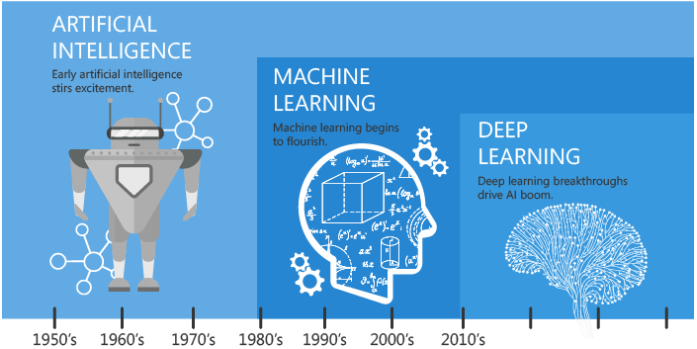
\includegraphics[scale=0.8]{images/AI_ML_DL.png}
		\end{center}
		\caption{Dezvoltarea inteligenței artificiale\newline
			\hspace{\linewidth}https://towardsdatascience.com/artificial-intelligence-vs-machine-learning-vs-deep-learning-2210ba8cc4ac/}
		\label{fig:AI_ML_DL}
	\end{figure}
	
	Așa cum se observă în Figura \ref{fig:AI_ML_DL}, putem afirmă că inteligența artificială este un termen mai vast care cuprinde celelalte două subcategorii. Aplicațiile care utilizează acest tip de tehnologie imită funcțiile cognitive pe care oamenii le asociază cu mințile umane, cum ar fi învățarea sau rezolvarea anumitor probleme.
	
	Machine learning înglobează algoritmii clasici pentru diferite tipuri de sarcini, precum regresia sau clasificarea. Acești algoritmi sunt dependenți în permanență de datele utilizate în procesul antrenării. Cu cât sunt mai multe date și cu cât aceste date sunt mai relevante pentru problema care încearcă să se soluționeze, randamentul acestora va crește. Antrenarea lor reprezintă cel mai important pas, deoarece în acest proces, se presupune minimizarea funcției de eroare (loss function). Rolul acesteia este de a stabili valorile de adevăr între ce a fost prezis, și adevărata clasă a datelor respective. În raport cu răspunsul funcției de eroare în cauză, anumite valori denumite greutăți (weights) vor fi actualizate.
	
	În învățarea automată există două categorii de date din care se poate învăța: date etichetate și date neetichetate. În prima categorie, atât parametrii de intrare cât și cei de ieșire sunt într-o formă ușor de citit pentru mașină, fiind nevoie de o cantitate mare de timp pentru a putea eticheta. În cazul datelor neetichetate, este nevoie de o soluție mai complexă pentru a putea utiliza acele informații. Astfel, reies la suprafață trei tipuri de învățare în machine learning:
	\begin{itemize}
		\item Învățare supervizată: este una din cele mai de bază tipuri de învățare automată. Chiar dacă este antrenat cu date etichetate, acest gen de învățare este unul foarte puternic. Se folosește un set de date (sau o parte din acest set de date, în general referindu-ne ca set de antrenare), care servește algoritmului cu scop de pregătire, iar alt set de date pentru a testa performanțele modelului.
		\item Învățare nesupervizată: principalul avantaj al acestei categorii este capacitatea algoritmilor de a lucra cu seturi de date neetichetate, eficientizând timpul programatorului. Permit astfel algoritmilor să exploreze și să găsească diferite șabloane și asocieri în seturile de date.
		\item Învățare prin "întărire" (reinforcement): se inspiră direct din modelul în care ființele umane învață din experiențele din viața de zi cu zi. Dispune de un algoritm care se îmbunătățește pe sine și învață din situații noi folosind o metodă de "încearcă și greșește" (în engleză trial and error). Rezultatele favorabile sunt încurajate sau "întărite", iar rezultatele greșite sunt descurajate sau "pedepsite".
	\end{itemize}
	
	Referitor la Figura \ref{fig:AI_ML_DL}, se poate constanta că machine learning este un domeniu destul de îmbătrânit, care încorporează metode și algoritmi, precum: Naive Bayes Classifier, Support Vector Machine, Random Forest. 

	Recent, în industria inteligenței articiale, a apărut conceptul de deep learning, care asamblează rețele artificiale neurale cu mai multe straturi. Deep learning poate fi definit ca un subset al învățării automate, care încearcă rezolvarea problemelor mai complexe prin găsirea unor diferite șabloane (pattern-uri) în date, acestea pentru oameni fiind insesizabile cu ochiul liber.

	Avantajul pe care îl aduc aceste tipuri de rețele față de cele tradiționale, este dat de eliminarea necesității de a extrage caracteristici din cadrul setului de date. Rezultatul extragerii caracteristicilor din setul de date definește o reprezentare abstractă a datelor. Acest proces este de obieci destul de complicat, care necesită cunoștințe detaliate în aria specifică a problemei care se încearcă soluționarea. Pasul extragerii trebuie revizuit de multiple ori, testat și rafinat pentru a obține rezultate optime.
	
	\clearpage
	
	\begin{figure}[h]
		\begin{center}
			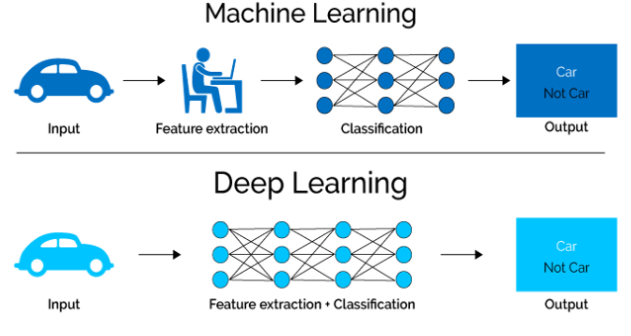
\includegraphics[scale=0.7]{images/ML_DL.png}
		\end{center}
		\caption{Analogie învățare automată și învățare profundă\newline
			\hspace{\linewidth}https://www.researchgate.net/figure/Comparison-between-ML-and-Dl-algorithm\_fig5\_344628869/}
		\label{fig:ML_DL}
	\end{figure}

	Pe de altă parte, în Figura \ref{fig:ML_DL}, se poate observa cum în cazul învățării profunde, pasul de extragere a caracteristicilor nu mai este necesar să fie executat de către programator, ci devine parte în procesul de antrenare a rețelei artificiale. Datele sunt brute și abstractizate astfel încât să poată fi memorate de diversele straturi ale algoritmului inteligent. Această reprezentare comprimată a datelor de intrare este utilizată pentru a construi rezultatul.

	Cu ajutorul rețelelor neurale profunde, acestea au făcut posibilă înțelegerea a seturilor de date complexe, precum semnalul audio reprezentând vocea umană, expresiile faciale și textul asociat cu fraze. Datele de antrenare folosite (care vor fi prezentate în capitolele următoare), sunt etichetate, făcând astfel posibilă identificare emoțiilor și a personalității candidatului. În secțiunea următoare, vom prezenta în mod minimalist modelele utilizate în aplicație:
	\begin{itemize}
		\item Rețele neurale convoluționale
		\item Rețele neurale recurente
	\end{itemize} 

	\clearpage
	\subsubsection{Rețele neurale convoluționale}
	O rețea neurală convolutională este un de algoritm inteligent care face parte din clasa modelelor deep learning. În general folosite în vederea artificială (computer vision), CNN (convolutional neural network) primește ca date de intrare, în majoritatea cazurilor, imagini (sau date care au fost structurate sub forma imaginilor), iar în urmă diferitelor operațiuni, se vor găsi pattern-uri în datele de antrenare, nevizibile unei persoane în mod natural. Sunt distinse printre alte tipuri de modele datorită performanțelor ridicate cu date care provin din: imagini, vorbit 	sau semnal audio.
	
	Din punct de vedere structural, o rețea neurală convolutională este alcătuită din următoarele componente:
	\begin{itemize}
		\item \textbf{Date de intrare}: cum este menționat mai sus, input-ul poate să provină din mai multe categorii, având și canale diferite de culori. Nu există o limită privind dimensiunea datelor, deoarece, scopul întregului proces este de a reduce dimensionalitatea, păstrând datele într-o formă compresată, fără pierderi de informații.
		\item \textbf{Strart(uri) de convoluție}: este elementul de bază al unei astfel de rețele, fiind locul în care majoritatea calculelor au loc. În funcție de dimensionalitatea datelor (matrici 2d sau 3d), va avea loc operația de convoluție, cu ajutorul unor măști (kernel). În urma acestui proces, se vor extrage anumite trăsături importante din cadrul datelor de intrare, care vor ajuta în determinarea apartenenței la o anumită clasă. De exemplu, printr-o speculație, putem considera din Figura \ref{fig:cnn}, în urma unui proces de convoluție, că se poate determina dacă piciorul mamiferului este sau nu al unei zebre. În urmă acestui proces, în funcție de numărul filtrelor, pasul (stride) și padding, se obțin hărți ale caracteristicilor (feature maps).
		\item \textbf{Strat(uri) de pooling}: au rolul de a reduce substanțial dimensiunea spațială, scăzând cantitatea de parametrii utilizați pentru calcule în rețea. Totodată, poate controla și "supra-adaptarea" (overfitting) rețelei. Printre tipurile de straturi de pooling, putem menționa următoarele:
		\begin{itemize}
			\item \textbf{Max pooling}: fiind cea mai comună abordare, deoarece oferă cele mai bune rezultate, max pooling va selecta elementul maxim din harta caracteristicilor (porțiunea filtrată de către mască)
			\item \textbf{Average pooling}: cum reiese și din nume, va selecta valoare medie din porțiunea filtrată de mască
		\end{itemize}
		\item \textbf{Strat(uri) de conectare}: sunt folosite cu scopul conectării neuronilor către stratul de ieșire, unde în funcție de valorile ponderilor fiecărui neuron în parte, se va putea face calculul posibilității apartenenței la o anumită clasă
	\end{itemize} 
	
	\clearpage
	\begin{figure}[h]
		\begin{center}
			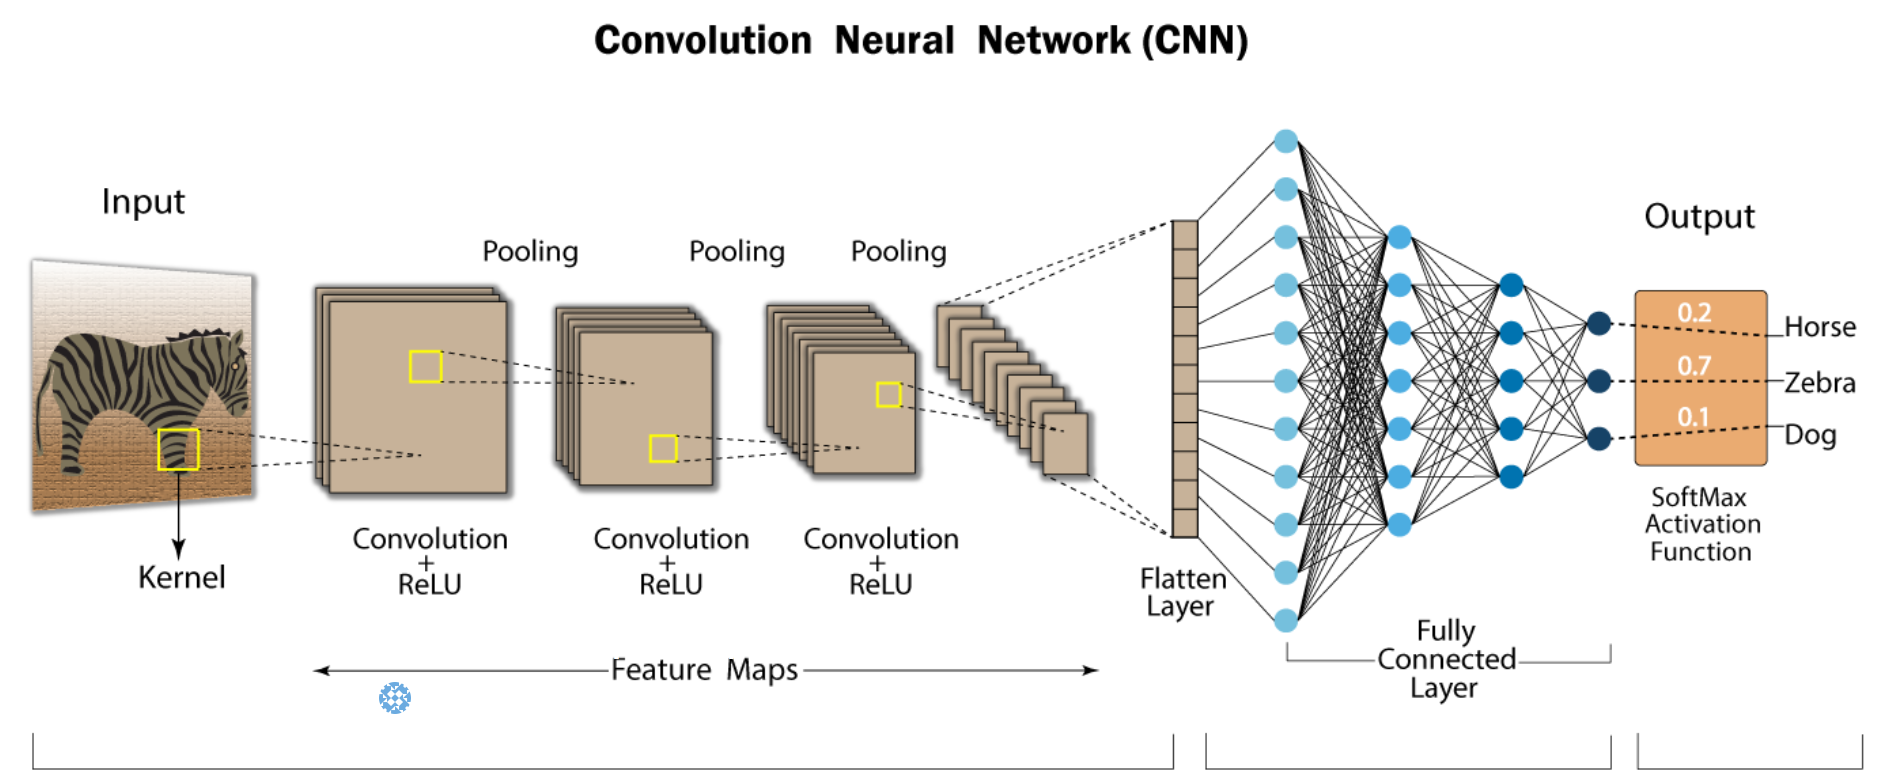
\includegraphics[scale=0.29]{images/cnn.png}
		\end{center}
		\caption{Rețea neurală convoluțională\newline
			\hspace{\linewidth}https://developersbreach.com/convolution-neural-network-deep-learning/}
		\label{fig:cnn}
	\end{figure}
	
	Împreună cu informațiile pe care le-am dobândit în urmă prezentării legate de rețelele neurale convolutionale, putem comenta asupra Figurii \ref{fig:cnn}. Din datele folosite pentru antrenare, filtrele aplicate succesiv ne vor ajută să găsim caracteristici. Transmise mai departe către stratul conectat, se va putea face interpretarea rezultatului, în funcție de gradul de apartenența la fiecare clasă în parte. Rezultatul va fi exprimat în procentaj, iar output-ul cu procentajul cel mai ridicat va exprima clasa decisă.
	
	În contextul aplicației "Multimodal Emotion Detection", acest tip de algoritm a fost utilizat cu preponderență în cazul identificării emoțiilor fluxul video. Prin intermediul acestor rețele, în imaginile procesate din input-ul video se vor găsi diferite asemănări, neuronii excitându-se atunci când un șablon recunoscut este detectat, fiind posibil ca emoțiile candidatului unui interviu să fie recunoscute. 
	
	\clearpage
	\subsubsection{Rețele neurale recurente}
	Rețelele neurale recurente sunt un tip robust de rețea neurală, folositoare pentru procesarea datelor secvențiale, ordinea lor având importantă. Derivate din rețelele cu propagare înainte (feedforward), RNN-urile (recurrent neural network) prezintă un comportament asemănător cu cel al creierului uman.

	La fel că ceilalți algoritmi de deep learning, rețelele neurale recurente sunt relativ vechi, fiind concepute în 1980, dar doar în ultimii ani a fost descoperit cu adevărat potențialul acestora. Creșterea în puterea computațională, accesul la cantități masive de date pe care le putem utiliza și apariția straturilor cu memorie lungă pe durata scurtă (long short-term memory), au adus RNN-urile în prim plan.

	După cum menționează Lex Fridman ("Ori de câte ori există o secvență de date temporale, unde conținutul spațial este mai important decât cel al fiecărui cadru individual"), rețelele neurale recurente au oferit suport pe parcursul lucrării pentru predicția datelor cu strânsă legătură temporală. Aceste rețele și-au îndeplinit scopul în aplicația "Multimodel Emotion Recognition" deoarece atât datele audio cât și cele scrise depind de ordinea lor în timp.

	Datele secvențiale sunt doar date ordonate în funcție de un anumite criteriu. Spre exemplu, putem menționa că date secvențiale, datele financiare sau chiar secvența de ADN. Cele mai populare date secvențiale sunt reprezentate de către seria temporală, în care sunt enumerate în ordine cronologică. Datele provenite din vorbit, care sunt utilizate în aplicație pentru a prezice emoția, sunt adecvate acestei rețele datorită sortării cronologice standard.

	Pentru a înțelege arhitectură acestor rețele, trebuia mai întâi să avem cunoștințe referitoare la mecanismul utilizat de această rețea, propagarea înainte. Într-o rețea neurală feed-forward, informațiile se mișcă doar într-o singură direcție: de la stratul de intrare, prin straturile ascunse, până la nivelul de ieșire. Informația se deplasează direct prin rețea și nu atinge același un neuron de două ori. Rețelele simple nu au niciun mecanism de memorare, cu privire la intrarea pe care o primesc, fiind slabe în a prezice ce urmează. Într-un RNN, informația circulă sub formă unei bucle. Când se ia o decizie, se va evalua input-ul curent cât și ce a învățat din experiențele anterioare.
	
	\begin{figure}[H]
		\begin{center}
			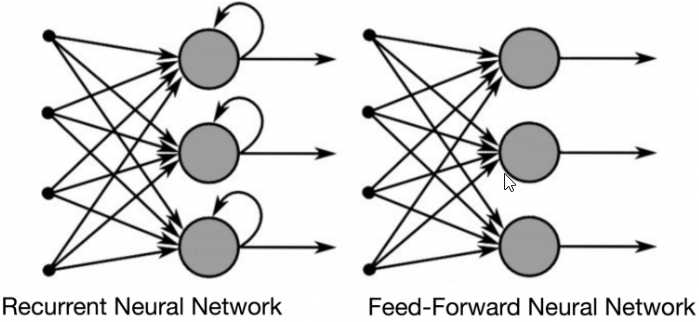
\includegraphics[scale=0.47]{images/fwd_recc.png}
		\end{center}
		\caption{Propagare recurentă și înainte\newline
			\hspace{\linewidth}https://builtin.com/data-science/recurrent-neural-networks-and-lstm/}
		\label{fig:fwd_recc}
	\end{figure} 

	În Figura \ref{fig:fwd_recc}, este ilustrată diferența dintre fluxul de intrare într-o rețea neurala recurentă și o rețea cu propagare înainte.
	
	O rețea neurala feed-forward atribuie, că toți ceilalți algoritmi de deep learning, o matrice de ponderi care va fi aplicată asupra datelor de intrare, urmând mai apoi să producă rezultatul. Totodată, va avea loc procesul de propagare înapoi (back propagation) petru actualizarea ponderilor. 
	
	Propagarea înapoi este utilizată pentru a calcula gradientul unei funcții de eroare în raport cu ponderile unei rețele neurale. Algoritmul își parcurge calea înapoi prin straturile rețelei, calculând derivatele parțiale ale ponderilor. Această tehnică este folosită pentru a reduce marjele de eroare în timpul antrenamentului.
	
	Mai jost sunt listate diferențele dintre o rețea normală și una recurentă, în contextul celor două propagări:
	\begin{itemize}
		\item Propagarea înainte: în acest pas, RNN-ul va înainta prin aplicarea ponderilor și pentru datele anterior procesate
		\item Propagarea înapoi: o astfel de rețea modifică greutățile atât prin gradient descent cât și prin propagarea inversă în timp (back propagation through time)
	\end{itemize}
	
	Principalele neajunsuri în cazul acestor algoritmi au apărut datorită gradientului. Primul este denumit "Explozia gradientului" (Expploading Gradient) și apare în cazurile când se asignează valori semnificativ de mari pentru ponderi. Această este ușor rezolvabilă prin trunchierea/plafonarea acestuia. A două problemă o reprezintă "Gradientul care dispare" (Vanishing Gradient), care apare atunci când valorile gradienților sunt prea mici, iar modelul încetează să învețe ori o face într-un timp prea mare. Pentru a rezolva această problema, au fost introduse straturile LSTM (Long Short-Term Memory).
	
	LSTM sunt o extensie pentru RNN-uri, unde se prelungește durata memoriei interne. Sunt folosite că elemente de baza pentru straturile rețelelor recurente. LSTM-urile asociază încă un set diferit de ponderi folosit pentru a oferi un grad de importanță asupra datelor noi. În funcție de aceste ponderi, datele noi vor putea impacta sau nu pe cele deja existente.
	
	Aceste straturi oferă suport rețelelor recurente să-și "amintească" input-urile pentru o perioada mai lungă de timp. Funcționalitate lor este asemănătoare cu cea a unui calculator, având capabilități de citire, scriere sau ștergere. Această memorie poate fi privită precum o celulă cu porți, care decide dacă să stocheze informația, să o șteargă, în funcție de importanța pe care trebuie să o acorde.
	
	Antrenarea utilizând astfel de rețele poate deveni una costisitoare datorită cantităților mari de date și a complexității calculelor. Procesorul central devine depășit de această ușoare, iar timpul necesar antrenării pentru acești algoritmi poate crește. Soluționarea în acest caz vine prin utilizarea procesorului grafic, acolo unde placă video permite acest lucru.
	
	\clearpage
	\subsubsection{Antrenare utilizând procesorul grafic}
	Procesorle grafice (graphical proccesing unit), dezvoltate inițial pentru accelerarea procesării grafice, pot îmbunătăți performanțele calculelor realizate într-o rețea neurala cu mai multe straturi. Au devenit o parte esențială a  infrastructurii inteligenței artificiale, iar procesoarele grafice noi au devenit specializate în acest domeniu.
	
	Principalul beneficiu al utilizării procesorului grafic este dat de paralelizarea sau procesarea simultană a datelor. Există patru tipuri de arhitecturi folosite pentru procesarea datelor în mod pparalel :
	
	\begin{itemize}
		\item Instrucțiune unică, date unice
		\item Instrucțiune unică, date multiple
		\item Instrucțiuni multiple, date unice
		\item Instrucțiuni multiple, date multiple
	\end{itemize}
	
	Scopul inițial al procesoarelor grafice erau pentru procesarea video, astfel solicitând utilizatorii să înțeleagă limbaje specifice precum OpenGL. În 2007, odată cu lansarea framework-ului NVIDIA CUDA \cite{cuda}, aria utilizării procesoarelor grafice a fost extinsă. CUDA se bazează pe limbajul de programare C și oferă un API (application programmin interface) pe care dezvoltatorii îl pot folosi pentru a aplica puterea de computație oferită de placa video în sarcinile de machine learning.
	
	Odată ce NVIDIA a introdus CUDA, au fost dezvoltate mai multe framework-uri pentru învățarea profundă, precum PyTorch și TensorFlow. Aceste tehnologii se folosesc de capabilitățile oferite de CUDA, oferind o accesibilitate mai mare pentru implementările moderne de deep learning.
	
	Procesoarele grafice pot efectua calcule simultan. Acest lucru permite distribuirea proceselor de instruire și poate accelera semnificativ operațiile de învățare automată. Folosind numărul mare de nuclee, putem utiliza mai puține resurse fără a sacrifica eficiența sau puterea.
	
	Când se definește o arhitectură pentru rețelele deep learning, următorii factori pot influență decizia de a utiliza sau nu un procesor grafic:
	\begin{itemize}
		\item Lățimea bandei de memorie: datorită memoriei video dedicată (VRAM), GPU-urile pot oferi lățimea de bandă necesară pentru a acomoda seturi de date
		\item Dimensiunea setului de date: procesoarele grafice legate în paralel scalează mult mai rapid decât procesoarele centrale, permițând procesarea a unor seturi de date masiv din punct de vedere cantitativ
	\end{itemize}
	
	
	Datorită puterii de procesare a plăcilor grafice, modelele de deep learning folosite în aplicație au fost antrenate cu ajutorul procesorului grafic. Placă video utilizată în cauză este un GeForece RTX 2060 (ediția laptop), oferind 1920 procesoare CUDA și 240 procesoare Tensor.
	\clearpage

	\subsection{Procesare digitală de semnal}
	Aceste tehnici complexe de procesare au fost utilizate în aplicație pentru identificarea emoției din voce. Această procesare nu va identifica cuvintele rostite de candidat, ci va încerca în funcție de anvelopa acustică, să determina starea persoanei care este intervievată.

	În mod natural, vocea este transmisă urechii umane printr-o undă acustică care se deplasează prin intermediul aerului, cu viteză sunetului. Din momentul în care este înregistrată de către un microfon, sunetul este transmis printr-un fir ca un semnal electric care se deplasează cu viteză luminii. Pentru a face acest eveniment posibil, semnalul acustic generat de corzile vocale umane trebuie mai întâi transformat într-un semnal electric și apoi convertit într-o formă acustică, pentru a putea fi înțeles de către oameni. Semnalul electric convertit este în mod convențional într-o formă analogică. Adică este reprezentat ca o tensiune care variază continuu într-un interval dat (0 și 1). Datorată degradării semnalului electric în cazul stocării, a deplasării acestuia pe distanțe lungi sau a procesării de către un calculator, se preferă transformarea lui într-o formă digitală.

	Indiferent de domeniul utilizat (timpului sau frecventelor), următorii termeni prezentați mai jos vor ajută în înțelegerea procesului de identificare a emoțiilor:
	
  	\begin{itemize} 
  		\item Rata de eșantionare (Sample rate): reprezintă numărul de date (sample-uri) care sunt înregistrate într-o secundă. Cu cât avem rată de eșantionare mai mare, cu atât calitatea semnalului va fi mai ridicată. Spre exemplu, rata de eșantionare folosită în general pentru scrierea CD-urilor cu muzică este de 44.1 KHz (kilo Hertzi). Asta înseamnă că o dată la o secundă, 44100 de date sunt înregistrate, pe care le putem studia. 
  		\item Fereastră (Window): semnalul poate fi segmentat într-un numărul egal de sample-uri \item Numărul de linii spectrale: simbolizează numărul de frecvențe identificate în urmă transformării din domeniul timpului în cel al frecvențelor 
  	\end{itemize} 
 	 Datele inregistarte de către microfon se vor află în domeniul timpului. În această sferă, principalul neajuns este reprezentat de insuficiența de operații folositoare pe care le putem utiliza în identificarea emoțiilor vocii. Pentru a satisface cerințele necesare analizei sentimentelor din voce, vom efectua trecerea din domeniul timpului în cel al frecvențelor utilizând Transformată Fourier \cite{ft}. 
  
 	 \clearpage 
  	\subsubsection{Transformata Fourier} 
  	Fiind folosită în multiple domenii precum procesarea imaginiilor, studiul semnalelor (incluzând cele acustice), transformata Fourier este un procedeu matematic care ne ajută la trecerea unui semnal din domeniul timpului în cel al frecvențelor. Avantajul analizei în acest domeniu este dat gama diversificată de informații precum și de operații pe care le putem folosi. 
  	
  	O puternică unealtă matematică, transformata Fourier (Jean-Baptiset Joseph Fourier) asumă faptul că un semnal poate fi descompus ca o suma de sinusuri/cosinusuri.
	
	\begin{figure}[h]
		\begin{center}
			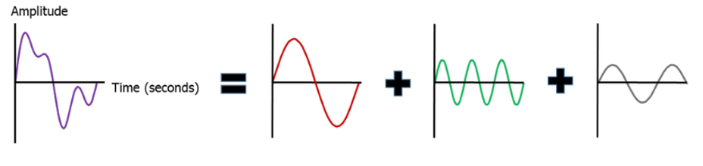
\includegraphics[width=\linewidth]{images/signals.png}
		\end{center}
		\caption{Semnal ca fiind o sumă de sinusuri\newline
			\hspace{\linewidth}https://community.sw.siemens.com/s/article/what-is-the-fourier-transform}
		\label{fig:singal_to_sinuses}
	\end{figure}

	Din Figura \ref{fig:singal_to_sinuses} se poate observa cum un semnal definit de amplitudine și timp, poate fi descompus într-o sumă de sinusuri, de frecvențe diferite.
	
	\begin{figure}[H]
		\begin{center}
			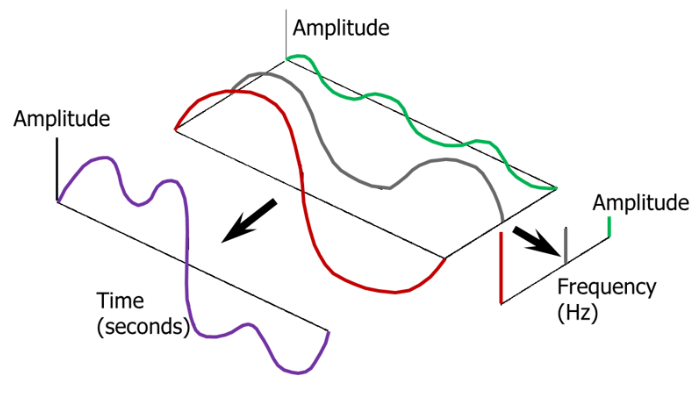
\includegraphics[scale=0.7]{images/FT_time_to_freq}
		\end{center}
		\caption{Domeniul frecvențelor \newline
			\hspace{\linewidth}https://community.sw.siemens.com/s/article/what-is-the-fourier-transform}
		\label{fig:signal_to_freq}
	\end{figure}

	Datorită motivelor enunțate în pagină anterioară care justifică necesitatea transformării în domeniul frecvențelor, vom explica acest fenomen cu ajutorul Figurii \ref{fig:signal_to_freq}. Putem observă că semnalul reprezentat de culoarea mov este compus din alte trei semnale. În urmă aplicării transformatei Fourier peste acest semnal, liniile spectrale vor reprezenta principalele frecvențe recunoscute.

	Din punct de vedere matematic, transformata Fourier este :
	\begin{equation}
		\label{ft_equation}
		S_x(f) = \int_{-\infty}^{+\infty} x(t)e^{-j2 \pi ft} dt
	\end{equation}
	
	unde $S_x(f)$ reprezintă frecvența măsurată în Hz iar $x(t)$ este semnalul în domeniul timpului. Rezultatul acestei operații este un număr complex (spre exemplu $a + bj$ este un număr complex întrucât a reprezintă partea reală iar b partea imaginară).
	
	\subsubsection{Transformata Fourier pe termen scurt}
	Adesea, transformata Fourier este evitată în a fi folosită în forma ei simplă în practică. Motivul este dat de variațiile prea bruște și multiple pe care semnalul le poate avea în domeniul timpului. Interpretarea unui semnal dintr-un singur segment devine problematică și costisitoare din punct de vedere al performanțelor. O soluție fezabilă este segmentarea semnalului în intervale mici, care mai apoi vor fi interpretate în mod individual. Această tehnică poartă numele de transformata Fourier pe termen scurt (short time Fourier Transform, STFT).
	
	\begin{figure}[H]
		\begin{center}
			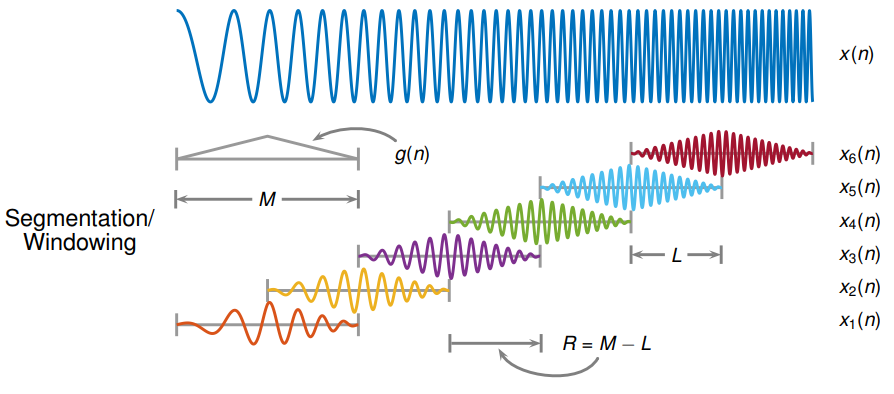
\includegraphics[width=\linewidth]{images/windowing.PNG}	
		\end{center}
		\caption{Domeniul frecvențelor \newline
			\hspace{\linewidth}https://nl.mathworks.com/help/signal/ref/stft.html}
		\label{fig:windowing}
	\end{figure}

	După cum se poate observa în Figura \ref{fig:windowing}, se aplică succesiv transformata Fourier pe segmente mici de date. Lungimea unui segment este aleasă în mod arbitrar, dar se recomandă să se folosească puteri ale lui 2, pentru a spori eficiența algoritmului. Acest proces este documentat ca fiind etapa de "windowing". O proprietate specială pe care o are acest procedeu este dat de intercalarea segmentelor. Prin utilizarea ferestrei în mod intercalat, vom avea posibilitatea de a obține valorile frecvențelor într-un mod mai determinist.
	
	\begin{figure}[H]
		\begin{center}
			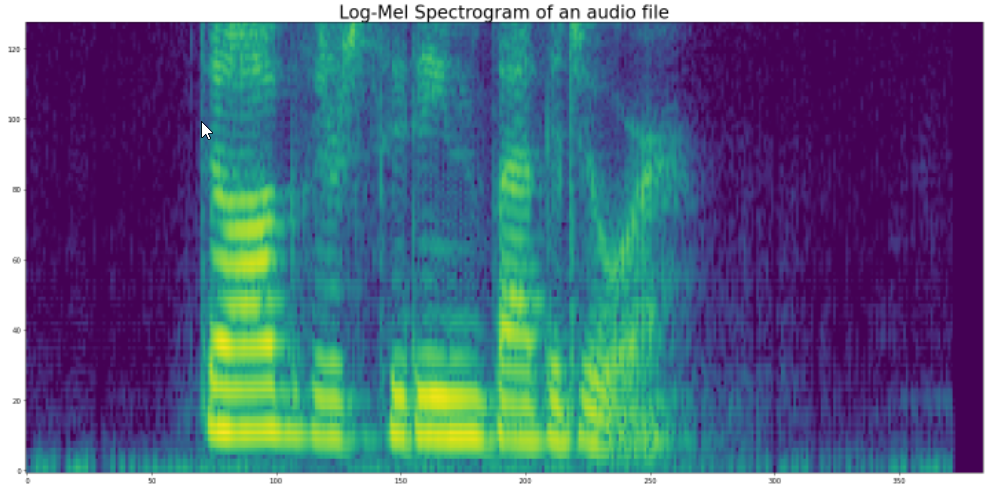
\includegraphics[width=\linewidth]{images/spectogram.PNG}	
		\end{center}
		\caption{Spectograma unui fișier audio folosit în antrenare}
		\label{fig:spectogram}
	\end{figure} 

	Rezultatul obținut în urmă aplicării transformatei Fourier pe termen scurt poate fi interpret sub formă unui grafic care poartă denumirea de spectogramă sau "waterfall" (cascadă). În exemplul din Figura \ref{fig:spectogram}, într-un spațiu cartezian XOY, axa OX reprezintă timpul iar cealaltă axa arată puterea lui. În funcție de intensitatea culorilor, putem determina degradarea precum și anvelopa acustică a semnalului sonor.
	
	\clearpage
	% diacritice
	\subsection{Tehnologii utilizate}
	"Multimodal Emotion Recognition" este o aplicație în care au fost folosite o serie de tehnologii. Aceste unelte fac posibilă atât navigarea printr-o interfață grafică prietenoasă utilizatorului, cât și cele mai importante funcționalități de bază, precum identificarea emoțiilor. Este o aplicație desktop, care oferă utilizatorului posibilitatea de a revizui un interviu, cu scopul identificării unor momente cheie, care au fost omise în procesul interviului.
	
	În funcție de cerințele și necesitățile aplicației, direcția aleasă în materie de tehnologii și limbaje de programare trebuie să fie una justificabilă. Așteptările construite în faza de proiecție, testare sau design trebuiesc menținute, iar rezultatul să fie sustenabil în raport cu tehnologiile alese pentru a realiza aplicația dorită. Primul pas înspre proiectare a fost alegerea unui limbaj de programare, care să satisfacă așteptările create. Această alegere poate deveni un grea, atunci când se ia în calcul beneficiile și dezavantajele fiecărui limbaj de programare. Având în vedere decizia care trebuie făcută, limbajele de programare se grupează în 2 categorii:
	\begin{itemize}
		\item Limbaje de nivel jos: sunt folosite pentru a scrie programe în raport la arhitectură și hardware-ul specific unui anumit tip de computer. Sunt aproape de limbajul nativ al unui calculator (binar), devenind astfel greu de înțeles de către programatori.
		Programele scrise în limbaje de nivel jos sunt rapide și eficiente din punct de vedere al memoriei. Acestea sunt utilizate în principal pentru a dezvolta sisteme de operare, drivere de dispozitiv, baze de date și aplicații care necesită acces direct la hardware. La rândul lor, se împart în două categorii: limbaj mașină și limbaj de asamblare.
		\item Limbaje de nivel înalt: sunt similare cu limbajul uman, prietenoase cu programatorii, ușor de scris, depanat și întreținut. Ele nu interacționează direct cu hardware-ul, ci mai degrabă, se concentrează cu operațiile complexe, eficientizarea scrisului de cod și lizibilitatea lui. Ca exemple, putem oferi: Python, Java, C\# etc. Programele concepute în limbaje de nivel înalt necesită compilator/interpretor (fiind la rândul ei un criteriu de clasificare) care să traducă codul sursă în limbajul mașinii. De asemenea, în funcție de paradigmă utilizată, limbaje de programare de nivel înalt se pot clasifică în: funcțională, procedurală și obiect orientată.
	\end{itemize}
	
	Acest program este conceput și scris în întregime utilizând limbajul de programare Python \cite{python}. Motivele care susțin decizia făcută sunt: capabilitatea de a programa în diferite paradigme (folositoare în etapă explorării și testării unor funcționalități), compatibilitatea cu majoritatea platformelor și a sistemelor de operare precum și accesul la o multitudine de biblioteci care au ajutat in cadrul dezvoltării aplicației.
	
	\clearpage
	\subsection{Python}
	Python este un limbaj de programare care face partea din categoria limbajelor interpretate. Aparitia acestui limbaj are loc la sfarsitul anului 1980 iar prima lansarea oficiala se intampla in 1991, fiind utiliza intern in cadrul companiei Google. Printre valorile utilizate, creatorul acestui limbaj, Guido van Rossum, abordeaza usurinta interpretarii codului, favorizand un stil identare fata cel folosind parantezele.
	
	Oferind suport pentru multiple paradigme de programre (functionala, procedurala si obiect orientata), python utilizeaza ca alte limbaje de nivel inalt un mecanism numit "garbage collector". Cu ajutorul acestui sistem, programatorul scapa de necesitatea eliberarii in mod manual a memoriei utilizate in timpul executiei programului. Acesta functie, gestioneaza in mod automat zonele de memorie utilizate, iar printr-o interna, dealoca zona atunci cand aceasta nu mai este accesata. 
	
	Adesea, utilizat impreuna cu limbajul de programare python este un sistem care sa administreze pachetele instalate, mediile de lucru create precum si versiunea limbajului utilizata. Distributia Anaconda este un astfel de sistem, avantajos de folosit atunci cand dorims sa lucram cu diferite pachete pentru manipularea datelor (nupmy, pandas) sau pentru invatarea automata (scikit-learn). Daca sunt nevoie de pachete suplimentare dupa instalarea acestei distributii, din aplicatia de administrare se pot instala manual bibliotecile necesare. O unealta folositoare care se instaleaza odata cu aceasta distrbutie este Jupyter Notebook. Este o aplciatie web folosita pentru rularea si editarea codului python, fiind executat local, fara a fi nevoie de acces la internet. Nucleul utilizat (kernel) faciliteaza rularea sucventiala a codului, facand posibila ca variabilele sa fie stocate si accesibile din memorie pe toata durata vietii. 
	
	\subsection{Qt}
	Qt (pronunțat cute) este un framework open-source de tipul GUI (graphical user interface), folosit în general pentru creare interfețelor grafice. Această tehnologie este realizată și inițial dedicată limbajului de programare C++. Însă, după o perioada de timp, s-a creat o interfață API, prin care codul Qt poate fi apelat și dintr-o manieră pitonică. Printre pachetele care oferă suport în acest sens, putem menționa: PyQt, PySide (dezvoltat de Qt Company). 

	Printre uneltele puse la dispoziție de către Qt, Qt Desginer a facilitat crearea interfeței grafice într-o manieră interactivă și dinamică. Această aplicație grafică ne pune la îndemna o serie funcționalități pentru adăugare de diverse elemente, cu ajutorul cărora putem construi o fereastră dorită. După cum se poate observă în Figura \ref{fig:qt_designer}, în panoul din stânga avem acces la o multitudine de "widget"-uri, fiecare dintre ele având un comportament și aspect diferit. Acestea sunt principalele componente pe care le putem folosi pentru a crea un window, dar Qt ne pune la dispoziție și un modul, prin care utilizatorul își poate crea elementele propii într-o mod customizabil.
	
	\begin{figure}[H]
		\begin{center}
			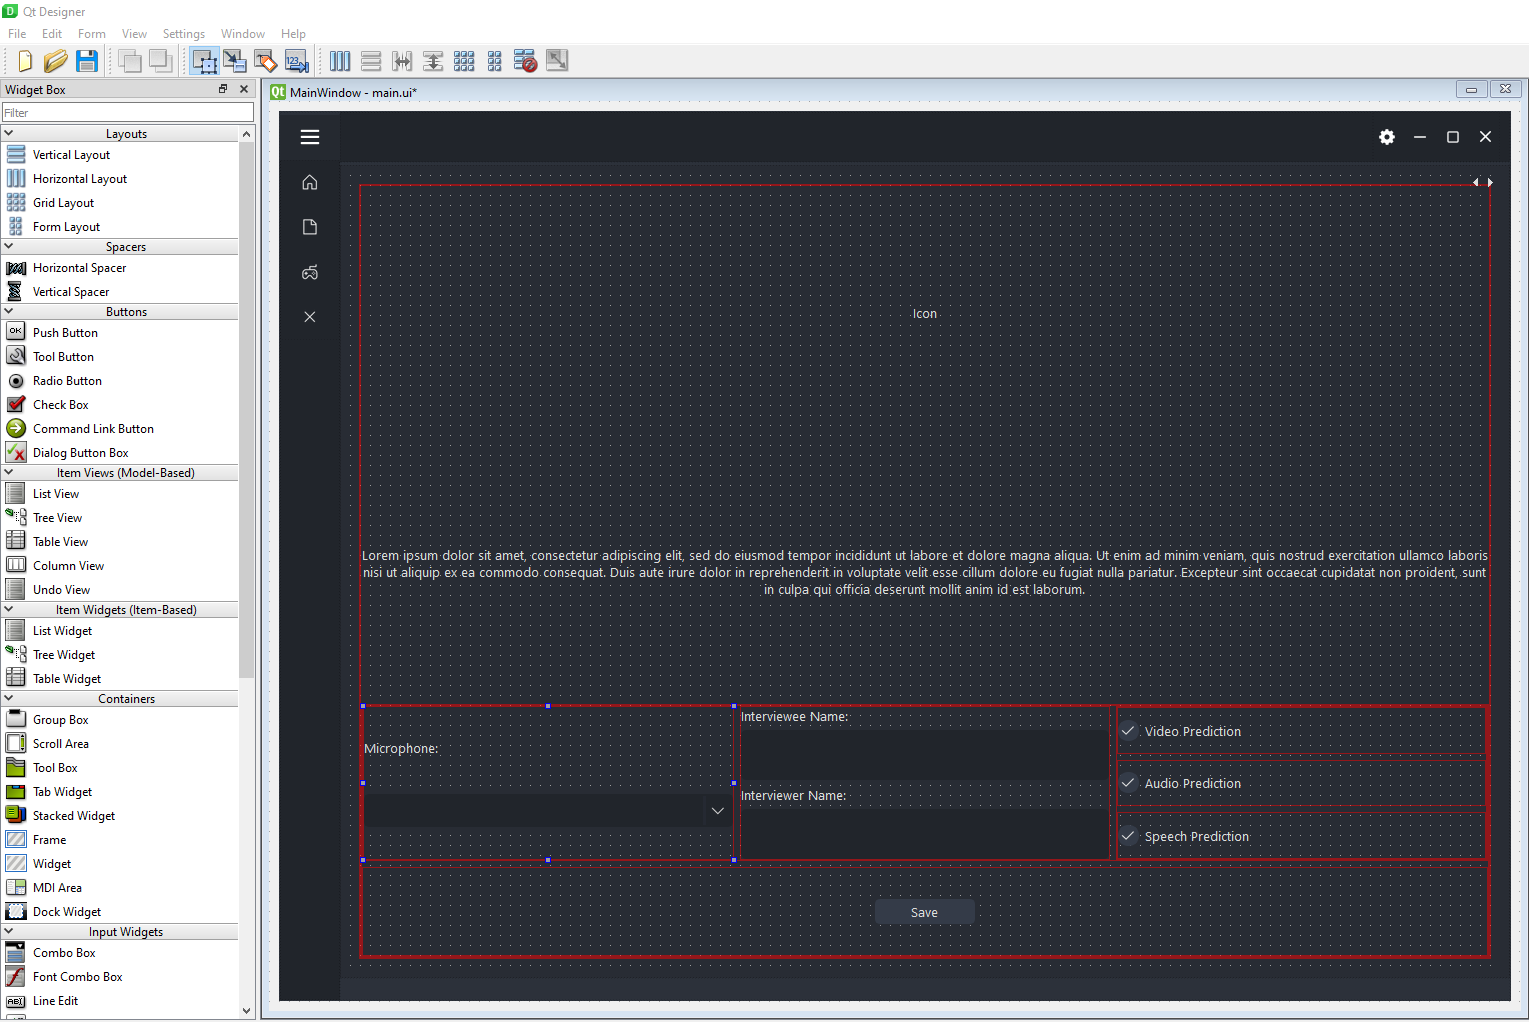
\includegraphics[scale=0.4]{images/qt_designer.png}
		\end{center}
		\caption{Qt Designer}
		\label{fig:qt_designer}
	\end{figure} 

	Printre principalele elemente utilizate preponderent în aplicație, le vom menționa pe următoarele (precum și informații referiatoare la utilizarea lor în implementarea curentă):
	\begin{itemize}
		\item Aspect (layout): acest element este folositor atunci când se dorește organizarea elementelor copil după anumite reguli. Ce le mai utilizate layout-uri sunt:
		\begin{itemize}
			\item Tip vertical: așezarea widget-urile copii va avea loc într-o manieră verticală, ca o stivă;
			\item Tip orizontal: constrânge ca widget-utile copii să fie așezate, în funcție de direcția aleasă, într-un mod longitudinal;
			\item Tip grilă: în funcție de dimensiunea aleasă, fiecare element copil utilizat în acest aspect va fi așezat într-un mod tabelar;
		\end{itemize}
		\item Elemente interactive:
		\begin{itemize}
			\item Buton: element de baza în aplicație, prin suprascrierea comportamentului unui buton, a fost posibilă interacționarea cu funcțiile aplicației (recunoașterea emoțiilor, suspendarea acestui proces sau oprirea);
			\item Casetă cu alegere: în general utilizat atunci când se dorește că utilizatorul să aleagă între variante multiple;
			\item Check box: folositor pentru valori binare (adevărat sau fals);
			\item Glisor: acest element ne va ajută pentru derularea interviului salvat, în momentul în care se dorește vizualizarea lui;
			\item Zona de text: utilizate pentru a oferi candidatului capacitatea de a-și introduce numele;
			\item Eticheta: diferite informații legate la starea aplicației;
			\item Tabel: folosit atunci când se dorește vizualizarea rapoartelor salvate
		\end{itemize}
	\end{itemize}
	
	\subsection{Biblioteci utilizate}
	
	
	\subsection{Șabloane de proiectare}
	
	%\bigskip
	
	\clearpage
    \printbibliography
    \clearpage
	\begin{figure}[H]
		\begin{center}
			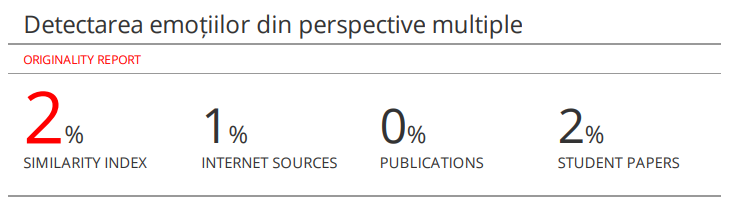
\includegraphics[scale=0.4]{images/plagiat.PNG}
		\end{center}
		\caption{Licență similaritate }
		\label{fig:sim}
	\end{figure} 	
\end{document}